\documentclass{article}
\usepackage{amsmath}
\usepackage{listings}
\usepackage{xcolor}
\usepackage{graphicx}
\usepackage{geometry}
\usepackage{hyperref}
\usepackage{tikz}
\usetikzlibrary{trees}
\geometry{margin=1in}

\title{Priority Queues and Heaps}
\author{}
\date{}

\definecolor{codegray}{rgb}{0.5,0.5,0.5}
\definecolor{backcolour}{rgb}{0.95,0.95,0.92}

\lstdefinestyle{cppstyle}{
  backgroundcolor=\color{backcolour},
  commentstyle=\color{codegray},
  keywordstyle=\color{blue},
  numberstyle=\tiny\color{codegray},
  stringstyle=\color{red},
  basicstyle=\ttfamily\footnotesize,
  breakatwhitespace=false,
  breaklines=true,
  captionpos=b,
  keepspaces=true,
  numbers=none,
  numbersep=5pt,
  showspaces=false,
  showstringspaces=false,
  showtabs=false,
  tabsize=2,
  language=C++
}

\begin{document}

\maketitle


A \textbf{priority queue} is an abstract data structure where each element has a priority. Elements are served based on priority rather than just order of insertion.

\textbf{Heaps} are a concrete implementation of priority queues. A heap is a complete binary tree satisfying the \textit{heap property}:
\begin{itemize}
  \item \textbf{Min-Heap:} Parent $\leq$ children
  \item \textbf{Max-Heap:} Parent $\geq$ children
\end{itemize}

\section{Use Case: Task Scheduling}

A heap can represent task priorities, where lower numbers indicate higher priority (Min-Heap). The following figure shows a binary Min-Heap storing integers:

\begin{center}
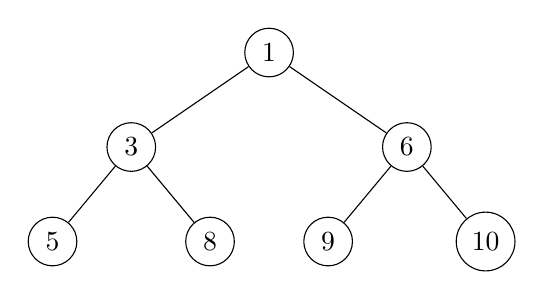
\begin{tikzpicture}[
  level distance=1.2cm,
  level 1/.style={sibling distance=3.5cm},
  level 2/.style={sibling distance=2cm},
  every node/.style={circle,draw}
]
\node {1}
  child {node {3}
    child {node {5}}
    child {node {8}}
  }
  child {node {6}
    child {node {9}}
    child {node {10}}
  };
\end{tikzpicture}
\end{center}

\textbf{Min-Heap Property:} Each parent node is less than or equal to its children.

\begin{itemize}
  \item Root node = minimum element
  \item Efficient for implementing priority queues
  \item Balanced due to complete binary tree structure
\end{itemize}

\section{Terminology}
\begin{itemize}
  \item \textbf{Heap:} Complete binary tree with ordering property
  \item \textbf{Priority:} Determines service order
  \item \textbf{Insert (Push):} Add element and restore heap
  \item \textbf{Extract (Pop):} Remove min/max and restore heap
\end{itemize}

\subsection{Array-Based Heap Representation}

A binary heap can be stored efficiently using a \textbf{zero-based array} without using explicit pointers. Given a node at index $i$, its position relative to other nodes is determined by:

\begin{itemize}
  \item \textbf{Left Child:} at index $2i + 1$
  \item \textbf{Right Child:} at index $2i + 2$
  \item \textbf{Parent:} at index $\left\lfloor \frac{i - 1}{2} \right\rfloor$
\end{itemize}

\textbf{Example:} For the array \texttt{[1, 3, 6, 5, 8, 9, 10]}  
This corresponds to the following binary Min-Heap:

\begin{center}
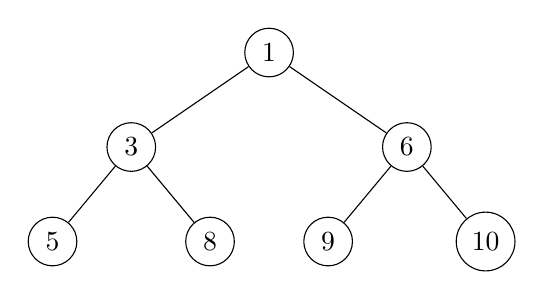
\begin{tikzpicture}[
  level distance=1.2cm,
  level 1/.style={sibling distance=3.5cm},
  level 2/.style={sibling distance=2cm},
  every node/.style={circle,draw}
]
\node {1}
  child {node {3}
    child {node {5}}
    child {node {8}}
  }
  child {node {6}
    child {node {9}}
    child {node {10}}
  };
\end{tikzpicture}
\end{center}

\textbf{Benefits of Array Representation:}
\begin{itemize}
  \item Compact memory layout—no pointer overhead
  \item Easy index arithmetic for navigation
  \item Suited for cache-efficient access
\end{itemize}

\textbf{Note:} 
Array-based heaps are limited to complete binary trees. They must be restructured or resized carefully during insertions and deletions to maintain the heap shape and property.

\section{C++ Implementation of a Min-Heap}

\begin{lstlisting}[style=cppstyle]
#include <iostream>
#include <vector>
#include <stdexcept>
using namespace std;

class MinHeap {
  vector<int> heap;

  // Moves a node up the tree until the heap property is restored
  void heapifyUp(int i) {
    // While node is not the root and its value is less than its parent
    while (i > 0 && heap[i] < heap[(i - 1) / 2]) {
      // Swap the node with its parent
      swap(heap[i], heap[(i - 1) / 2]);
      // Move to the parent index
      i = (i - 1) / 2;
    }
  }

  // Moves a node down the tree until the heap property is restored
  void heapifyDown(int i) {
    int n = heap.size();
    while (2*i + 1 < n) { // While at least one child exists
      int left = 2*i + 1;
      int right = 2*i + 2;
      int smallest = left;

      // Choose the smaller of the two children
      if (right < n && heap[right] < heap[left])
        smallest = right;

      // If the current node is smaller than both children, stop
      if (heap[i] <= heap[smallest])
        break;

      // Otherwise, swap with the smaller child
      swap(heap[i], heap[smallest]);
      i = smallest; // Continue at the child index
    }
  }

public:
  void insert(int val) {
    heap.push_back(val);          // Insert at the end
    heapifyUp(heap.size() - 1);   // Restore heap property
  }

  int extractMin() {
    if (heap.empty()) throw runtime_error("Empty heap");
    int minVal = heap[0];         // Root has the minimum value
    heap[0] = heap.back();        // Replace root with last element
    heap.pop_back();              // Remove last element
    heapifyDown(0);               // Restore heap property
    return minVal;
  }

  int peek() const {
    if (heap.empty()) throw runtime_error("Empty heap");
    return heap[0];               // Return root without removing
  }

  bool empty() const { return heap.empty(); }
};
\end{lstlisting}

\textbf{Usage:}
\begin{lstlisting}[style=cppstyle]
MinHeap h;
h.insert(5);
h.insert(2);
h.insert(8);
cout << h.extractMin(); // prints 2
\end{lstlisting}

\subsection{STL \texttt{priority\_queue}}

C++ STL provides a container adapter for priority queues backed by a heap.

\begin{lstlisting}[style=cppstyle]
#include <queue>
#include <vector>
using namespace std;

priority_queue<int> maxpq; // default: max-heap
priority_queue<int, vector<int>, greater<int>> minpq; // min-heap

minpq.push(4);
minpq.push(1);
cout << minpq.top(); // prints 1
minpq.pop();         // removes 1
\end{lstlisting}

\section{Time Complexities}
\begin{itemize}
  \item \textbf{Insert:} $\mathcal{O}(\log n)$
  \item \textbf{Extract-Min/Max:} $\mathcal{O}(\log n)$
  \item \textbf{Peek:} $\mathcal{O}(1)$
  \item \textbf{Build-Heap (from array):} $\mathcal{O}(n)$
\end{itemize}

\subsection*{Why Are Heap Operations $O(\log n)$?}

A binary heap is a complete binary tree stored as an array. Its height is $\log n$ (base 2), since each level doubles the number of nodes.

Operations like \texttt{insert}, \texttt{extract-min}, or \texttt{decrease-key} involve traversing from a leaf to the root or vice versa, adjusting positions to maintain the heap property. These traversals take at most $\log n$ steps, resulting in $O(\log n)$ time complexity.

\section{Practice problem}
Leetcode Problem 295: \textit{Find median from data stream}

\url{https://leetcode.com/problems/find-median-from-data-stream/description/}

\end{document}